Рассмотрим работу алгоритмов на словаре, где каждый элемент имеет следующую структуру: $key$ -- ключ, $value$ -- значение. Длина словаря -- $len$.

\section{Поиск полным перебором}
\qquadОсуществляется поэлементный проход по словарю, и на каждом шаге ключ сравнивается с ключём текущего элемента. Если значения совпали, значит, цель достигнула, элемент найден. В таком случае, алгоритм завершает свою работу. Если же до конца словаря совпадение не было найдено, делается вывод о том, что такого ключа нет.\\

\textbf{Схема} алгоритма представлена на Рис.\ref{fig1:image}.
\begin{figure}[h]
	\begin{center}
		{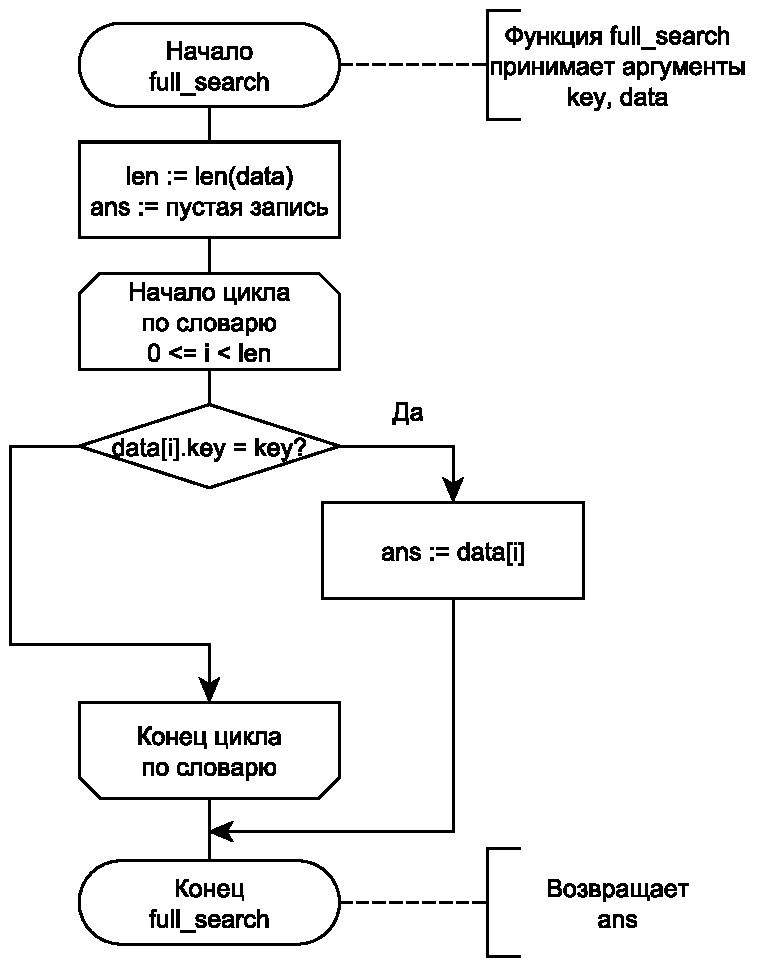
\includegraphics[scale = 0.6]{schemes/full}}
		\caption{Поиск полным перебором}
		\label{fig1:image}
	\end{center}
\end{figure}

\newpage
\subsection{Поиск в упорядоченном словаре двоичным поиском}
\qquadПеред применением алгоритма нужно предварительно отсортировать массив.
В двоичном поиске вводятся такие понятия как левая ($left$) и правая ($right$) границы массива, индексы которых хранятся в соответствующих переменных. В начале работы алгоритма индекс левой границы равен 0, а правой $len - 1$. На каждой итерации цикла вычисляется индекс элемента, с которым будет производиться сравнение ключа. Находится он по формуле \ref{formula1}.
\begin{equation}\label{formula1}
	middle = \frac{left + right}{2}
\end{equation} 

Если данный ключ больше значения, которое находится по индексу $middle$, то в таком случае левая граница принимает значение $middle + 1$, если меньше, то правая граница становится равной $middle - 1$. В случае совпадения, делается вывод, что нужное значение успешно найдено, и алгоритм завершает свою работу. Если же правая граница становится меньше левой, это свидетельствует о том, что такого ключа в словаре нет, и нужно завершать работу.\\

\textbf{Схема} алгоритма представлена на Рис.\ref{fig2:image}.
\begin{figure}[h]
	\begin{center}
		{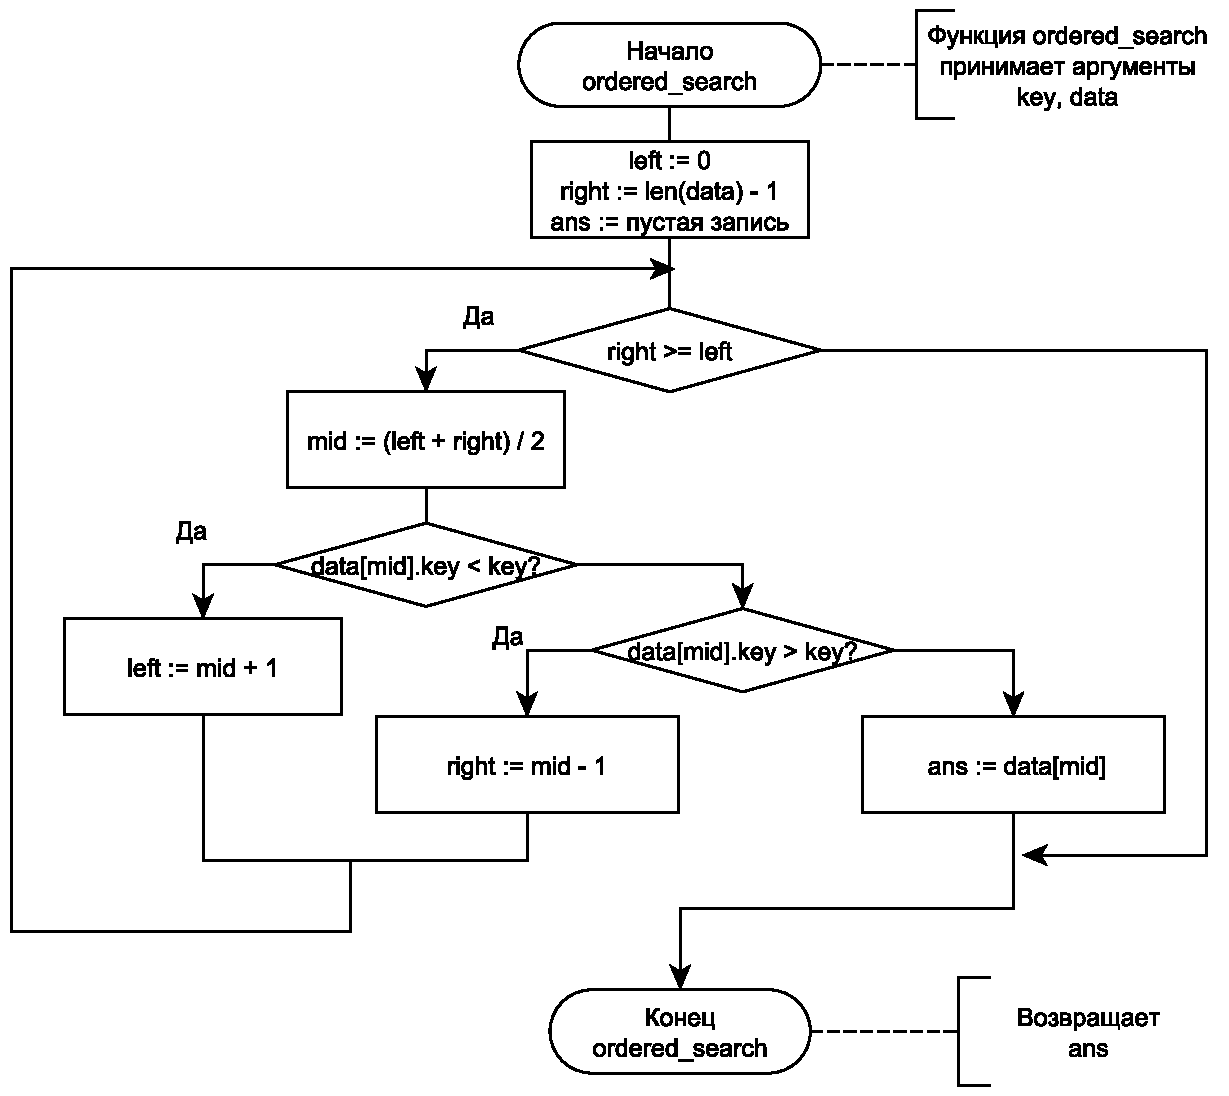
\includegraphics[scale = 0.6]{schemes/sort}}
		\caption{Поиск в упорядоченном словаре двоичным поиском}
		\label{fig2:image}
	\end{center}
\end{figure}

\subsection{Поиск полным перебором с использованием сегментов}
\qquadДля этого алгоритма также требуется предварительная подготовка -- разбиение словаря на сегменты. В данном случае словарь разбивается по частоте запросов. Так, экспериментально было выяснено, что в рассматриваемом словаре url, оканчивающиеся на $ru, com, io$, встречаются примерно одинаковое количество раз,  в то время как $net, biz, org, info$ употреблены в два раза меньше. \\

На основе этого были выделены сегменты с ключами: $\left\{ ru \right\}, \left\{ com \right\}, \left\{ io \right\}, \left\{ net, biz \right\}, \left\{ org, info \right\}$. И на основе этих ключей словарь разделяется на соответствующие сегменты. Каждый из которых состоит из одного из ключей выше и массива элементов словаря (каждый элемент представляет из себя key : value).\\

\textbf{Схема} алгоритма разбиение на сегменты представлена на Рис.\ref{fig3:image}.\\

\newpage

\begin{figure}[pt!]
	\begin{center}
		{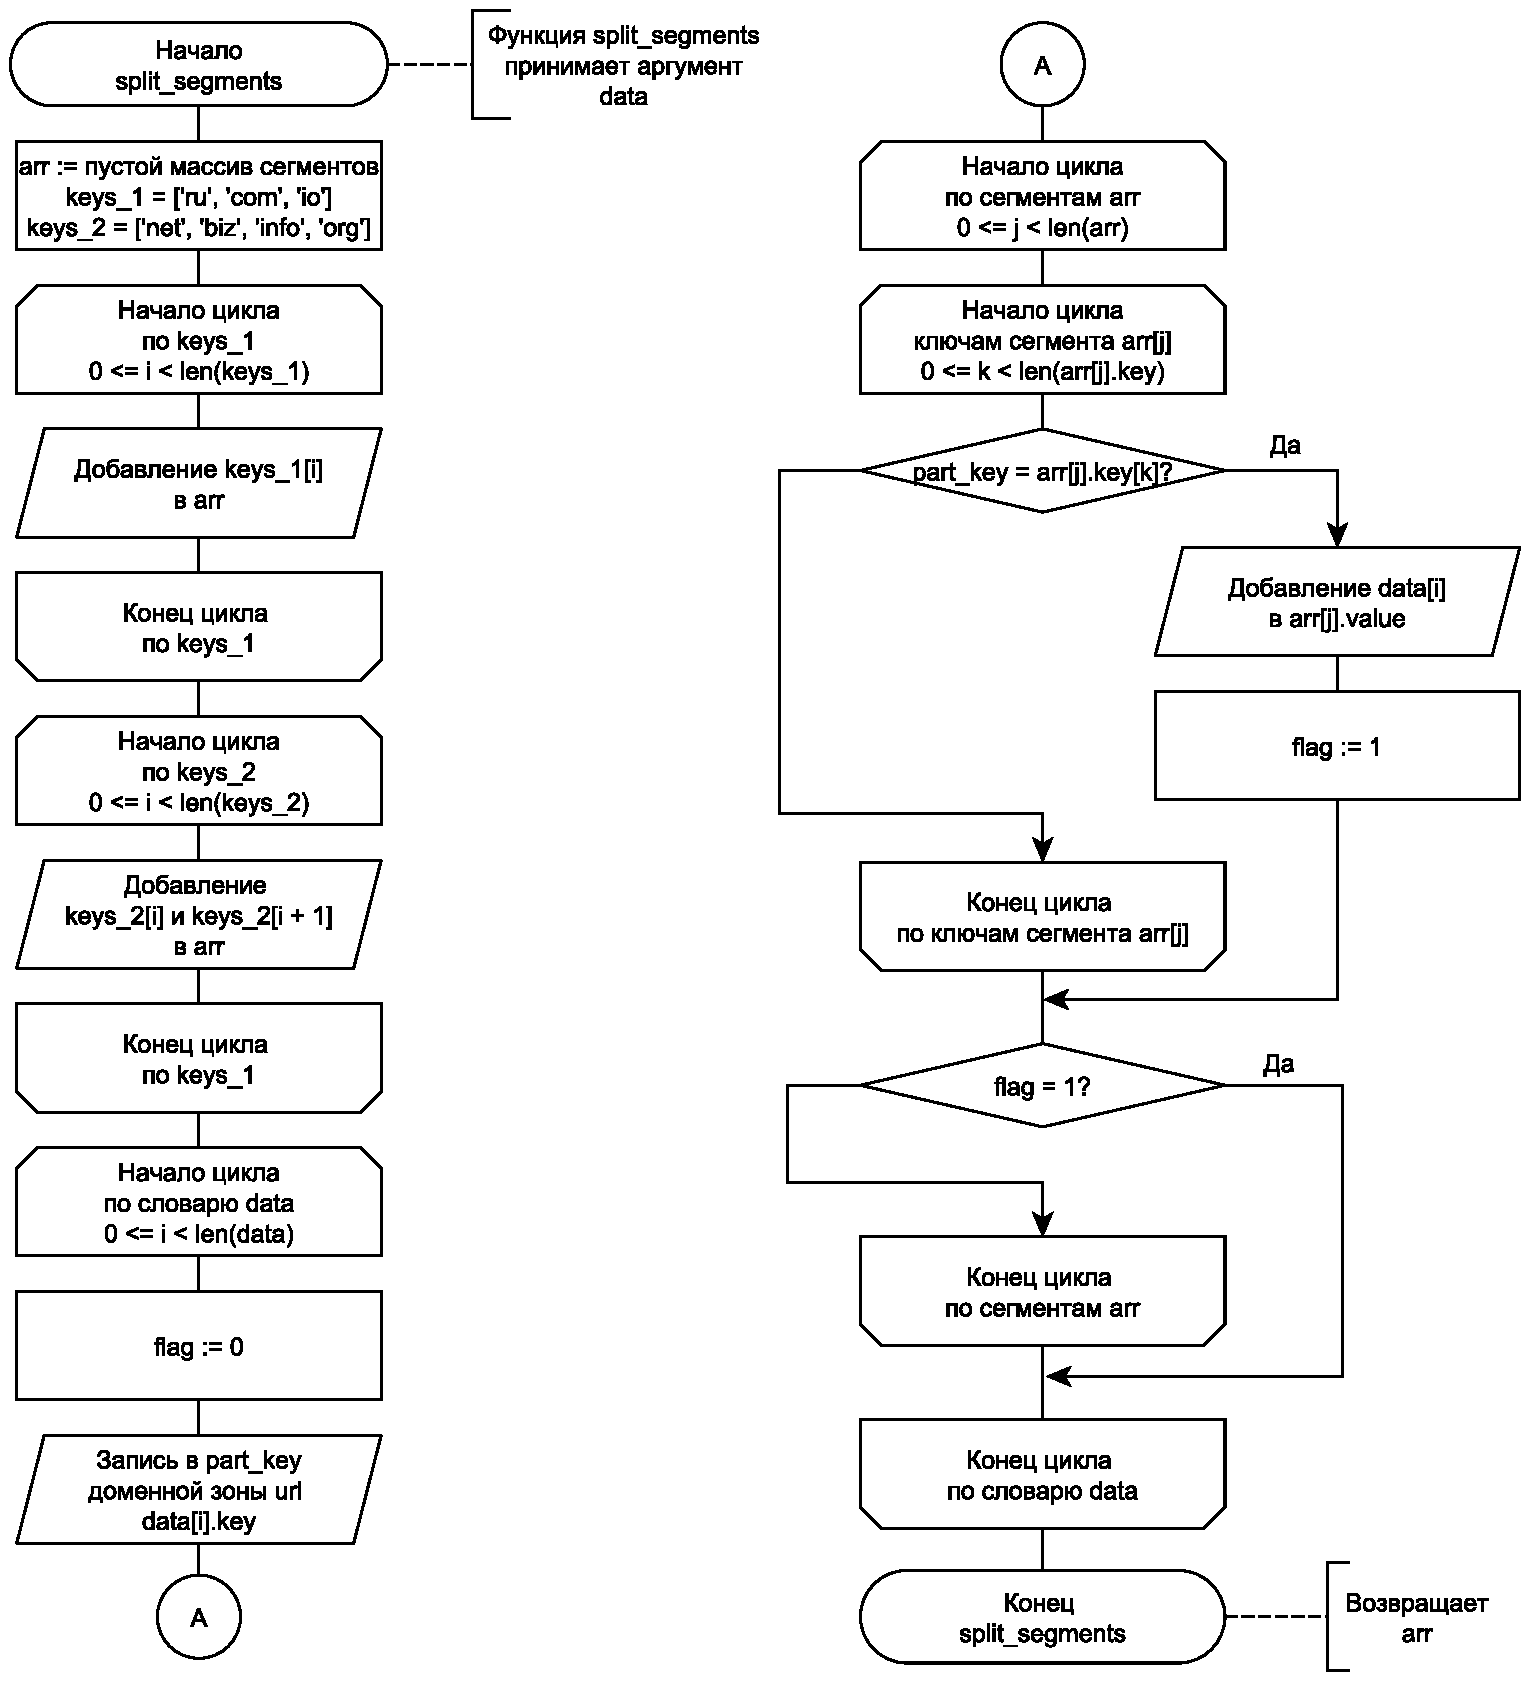
\includegraphics[scale = 0.6]{schemes/split}}
		\caption{Разбиение словаря на сегменты}
		\label{fig3:image}
	\end{center}
\end{figure}

В этом алгоритме сначала находится подходящий сегмент, затем уже внутри сегмента производится последовательный поиск ключа.\\

\textbf{Схема} алгоритма представлена на Рис.\ref{fig4:image}.

\begin{figure}[pt!]
	\begin{center}
		{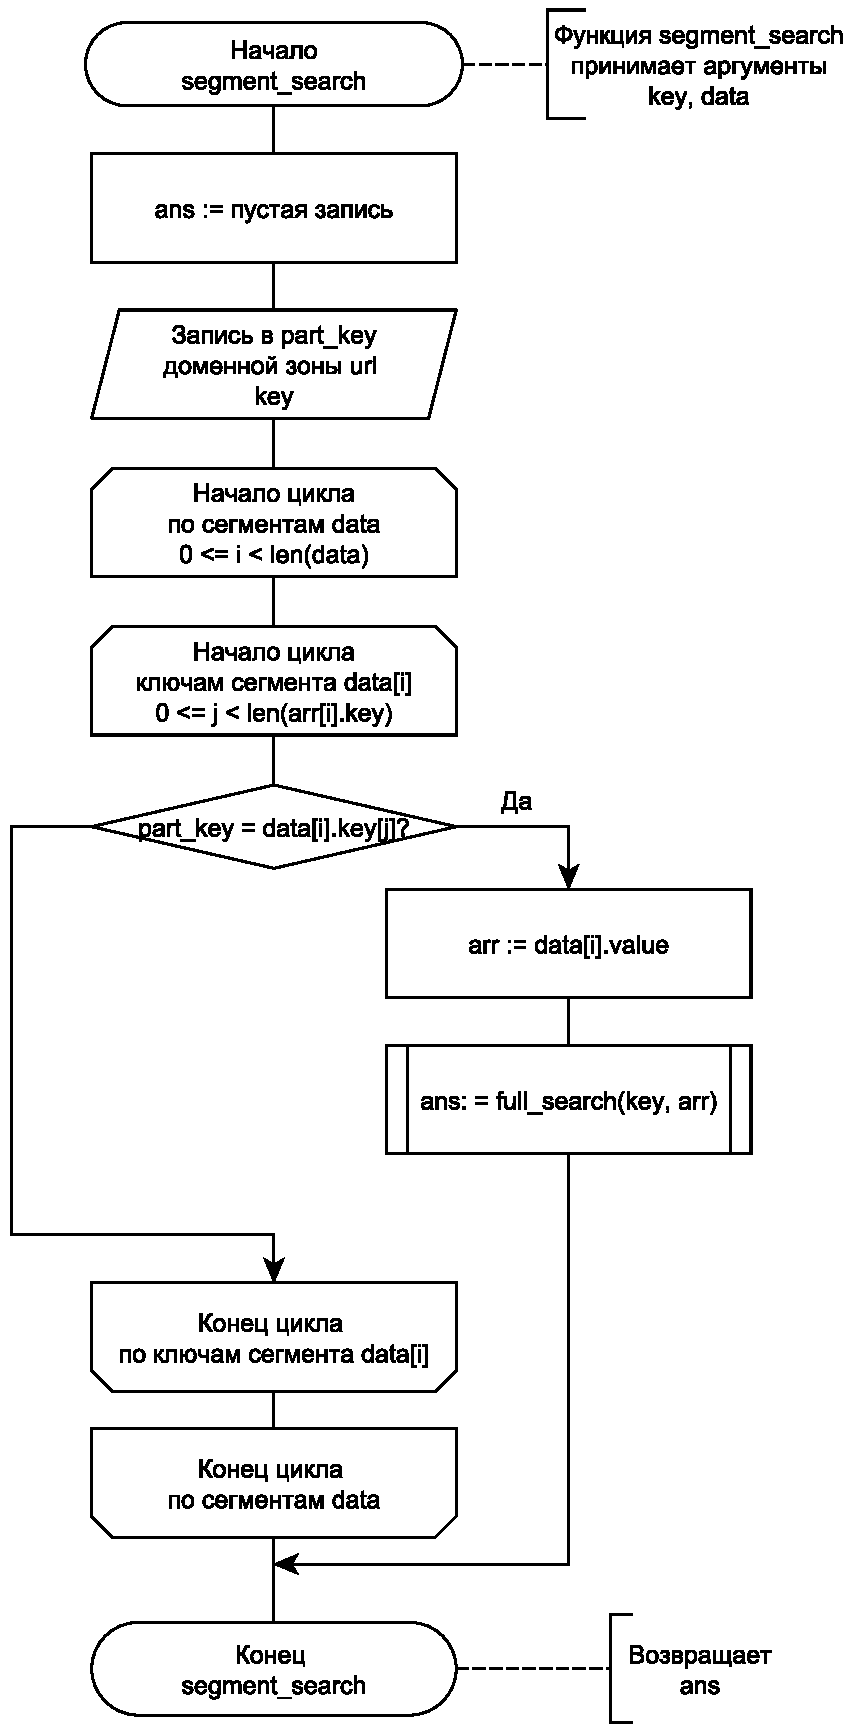
\includegraphics[scale = 0.6]{schemes/segments}}
		\caption{Поиск полным перебором с использованием сегментов}
		\label{fig4:image}
	\end{center}
\end{figure}

\section{Требования к ПО}
\qquadДля корректной работы алгоритмов и проведения тестов необходимо выполнить следующее.
\begin{itemize}
	\item Обеспечить возможность ввода ключа и выбора алгоритма через консоль.
	\item В случае ввода некорректных данных вывести соответствующее сообщение. Программа не должна аварийно завершаться.
	\item Реализовать возможность вывода на экран времени, затрачиваемое на поиск каждого ключа из словаря, а также несуществующего ключа. Вывести максимальное, минимальное и среднее значение.
\end{itemize}

\section{Заготовки тестов}
\qquadПри проверке на корректность работы необходимо провести следующие тесты:
\begin{itemize}
	\item поиск первого элемента словаря;
	\item поиск последнего элемента словаря;
	\item поиск каждого сотого элемента словаря;
	\item поиск несуществующего ключа.
\end{itemize}

\section*{Вывод}
\addcontentsline{toc}{section}{Вывод}
\qquadВ этом разделе разобраны основные принципы выбранных алгоритмов, приведены схемы работы каждого из них, сформулированы требования к программному обеспечению и сделаны заготовки тестов.
